\section{Canal de Voluntários}

A JCI é uma força tarefa que atua em vários países do mundo promovendo formas e oportunidades de se contribuir individualmente para o desenvolvimento social. 
Seu trabalho se dá com o preparo e reunião de pessoas interessadas em exercer serviços voluntários. A grande meta da organização é conquistar espaço como principal 
rede mundial de colaboradores recrutados. Para isso, seu crescimento vem através de representantes locais que surgem motivados por necessidades de suas regiões. 
A JCI Londrina existe dessa forma, empregando os princípios da JCI internacional com autonomia para captação de recursos e de desenvolvimento de soluções na ajuda
a ONGs locais.

Apesar da liberdade, esbarra-se em empecilhos para uma atuação eficiente do grupo. O recrutamento de voluntários depende de fatores instáveis, como disposição e 
idoneidade de pessoas aptas a ajudar. Nem sempre uma pessoa disposta é apta para as necessidades de uma entidade. Nem sempre uma pessoa apta e experiente está
disponível. Além do mais, entidades mais necessitadas muitas vezes não conseguem captar recursos em tempo hábil para suas atividades. Todos esses problemas estão 
relacionados com a pouca visibilidade de demandas de várias ONGs. Na média londrinense, um quarto dos colaboradores das entidades são voluntários, com os contratados
recebendo menos de R\$1000,00, e grande parte das entidades estão limitadas a um orçamento menor que R\$50000,00 contando com cerca de 10 funcionários. Todas as
organizações concorrem por uma atenção mal distribuída.

Devido a esses impasses, surgiu dentro da JCI Londrina uma proposta de ferramenta auxiliar para recrutamento de pessoal e de doadores, denominado Canal de
Voluntários. O projeto visa desonerar tanto a obtenção de recursos para toda ONG em situação de carência quanto o oferecimento de benefícios por qualquer pessoal
ou instituição. Através das tarefas já exercidas na JCI de orientação de indivíduos para voluntáriado, algumas informações relevantes já foram coletadas. Elas
expõem associações que formam perfis de voluntários, e contribuem fundamentalmente para o conceito da ferramenta auxiliar. Usadas para direcionamento de recursos
disponíveis, se a análise sobre essas informações for automatizada, as decisões tomadas serão mais eficientes e contarão com uma base mais sólida.

As expectativas a respeito da ferramenta envolvem, além do melhor uso de perfis traçados com necessidades demandadas, o incentivo a pessoas em, eficazmente,
manifestar interesse por ofertar voluntáriado e doações (através da facilitação e acessibilidade associadas à Internet), acompanhamento mais eficiente da 
longevidade das ONGS, aumento do grau de confiabilidade para um contato bem sucedido entre duas partes, e agilidade na contribuição com iniciativas assurgentes,
como projetos ou campanhas.

\newpage
\section{Diagrama de Atividades}

\begin{figure}[h]
  \begin{center}
    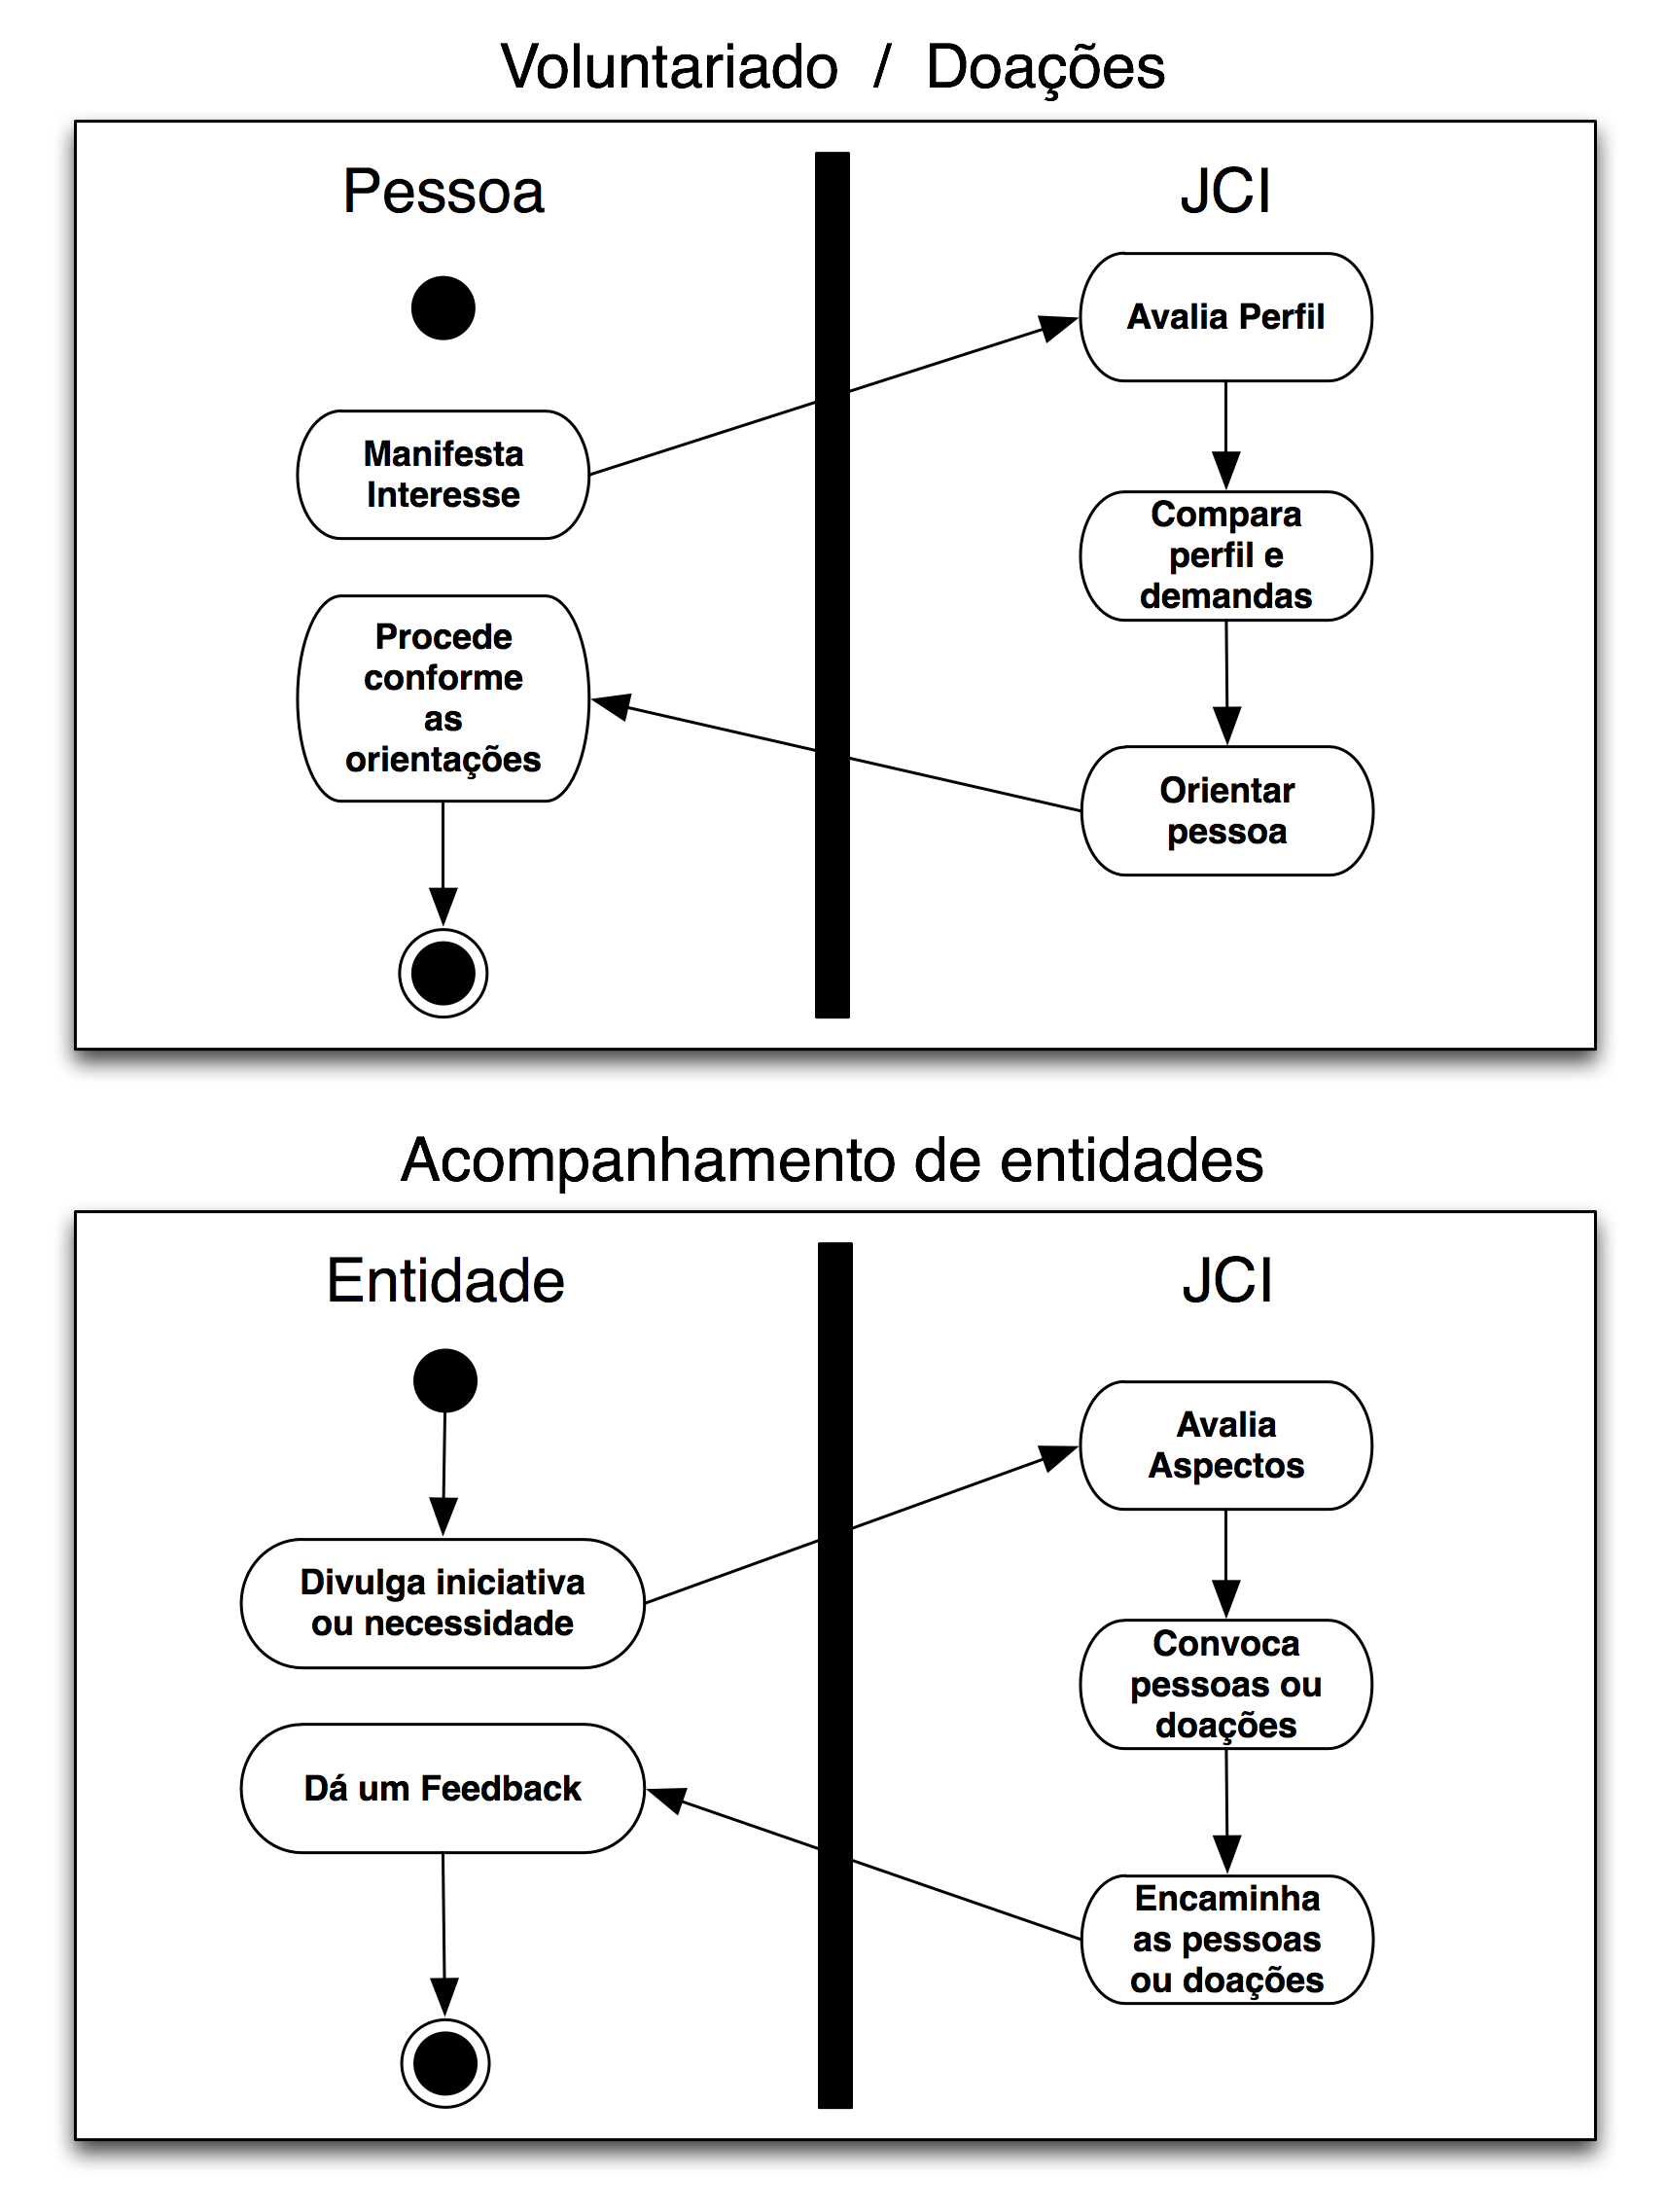
\includegraphics[scale=.195]{atv-neg.png}
   \end{center}    
\end{figure}
